\chapter{Metoda glavnih komponent}
Vektorji vhodnih uteži na sloju $N^{(i)}$ so velikosti $N^{(i - 1)}$. Te številke so običajno veliko večje od 2 ali 3, zato si teh vektorjev ne moremo predstavljati, kot točk v 2 oz. 3 dimenzionalnem prostoru. V tem poglavju si bomo pogledali linearno metodo za zmanjševanje dimenzij, ki se imenuje metoda glavnih komponent. Pri tem bomo sledili~\cite{shlens2014tutorial}.

\section{Sprememba baze}
Cilj metode glavnih komponent je zbirko podatkov predstaviti z bazo, katere bazni vektorji bodo po vrsti razkrili največ informacije o originalnih podatkih. Glavna ideja je, da bodo najpomembnejši bazni vektorji zadostovali za predstavo strukture podatkov, medtem ko bodo manj pomembnejši le filtrirali morebitne šume. Originalne podatke, ki smo jih predstavili z matriko $X$, bomo torej transformirali v matriko $Y$, ki bo predstavljala podatke zapisane v novi bazi. Vsak nov bazni vektor lahko zapišemo kot linearno kombinacijo originalnih baznih vektorjev, zato lahko poiščemo matriko linearne preslikave $P$, tako da bo veljalo:
\begin{equation}
  Y^T = PX^T
\end{equation}

\section{Napaka rekonstrukcije in varianca}
Vrednost podatkov v novi bazi dobimo s pravokotno projekcijo na nove normirane bazne vektorje. Iskanja nove komponente se lahko lotimo, tako da poiščemo enotski vektor $u_1$, ki bo po projekciji podatkov minimiziral napako rekonstrukcije originalnega prostora.
\begin{equation}
  E(u_1) = \sum_{i} \left\lVert x^{(i)} - (u_{1}^{T}{x}^{(i)})u_{1} \right\rVert^2
\end{equation}

\begin{figure}[H]
  \centering
  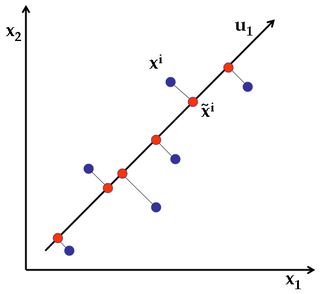
\includegraphics[width=0.7\linewidth]{resources/napakaRekonstrukcije.png}
  \caption{Napaka rekonstrukcije. Vir:~\cite{dataset}}\label{fig:error}
\end{figure}
\begin{comment}
https://www.google.com/url?sa=i&url=https%3A%2F%2Fstats.stackexchange.com%2Fquestions%2F194278%2Fmeaning-of-reconstruction-error-in-pca-and-lda&psig=AOvVaw2fogYikUFLgwt2PUiiO5BI&ust=1714336714385000&source=images&cd=vfe&opi=89978449&ved=0CBIQjRxqFwoTCNDVwoig44UDFQAAAAAdAAAAABAE
\end{comment}

To pa je ravno ekvivalenten problem iskanja vektorja, ki bo po projekciji originalnih podatkov jih ohranjal najbolj razpršene. Razpršenost merimo z varianco, ki je povprečna oddaljenost projekcije podatkov od projekcije središčne točke podatkov $\bar{x} = \frac{1}{m} \sum_{i} x^{(i)}$:
\begin{equation}
  \mathrm{Var}(u_1^{\top}X^{\top}) = \frac{1}{m} \sum_{i=1}^{m} \left(u_1^{\top}x^{(i)} - u_1^{\top}\bar{x}\right){}^2
\end{equation}
\begin{figure}[H]
  \centering
  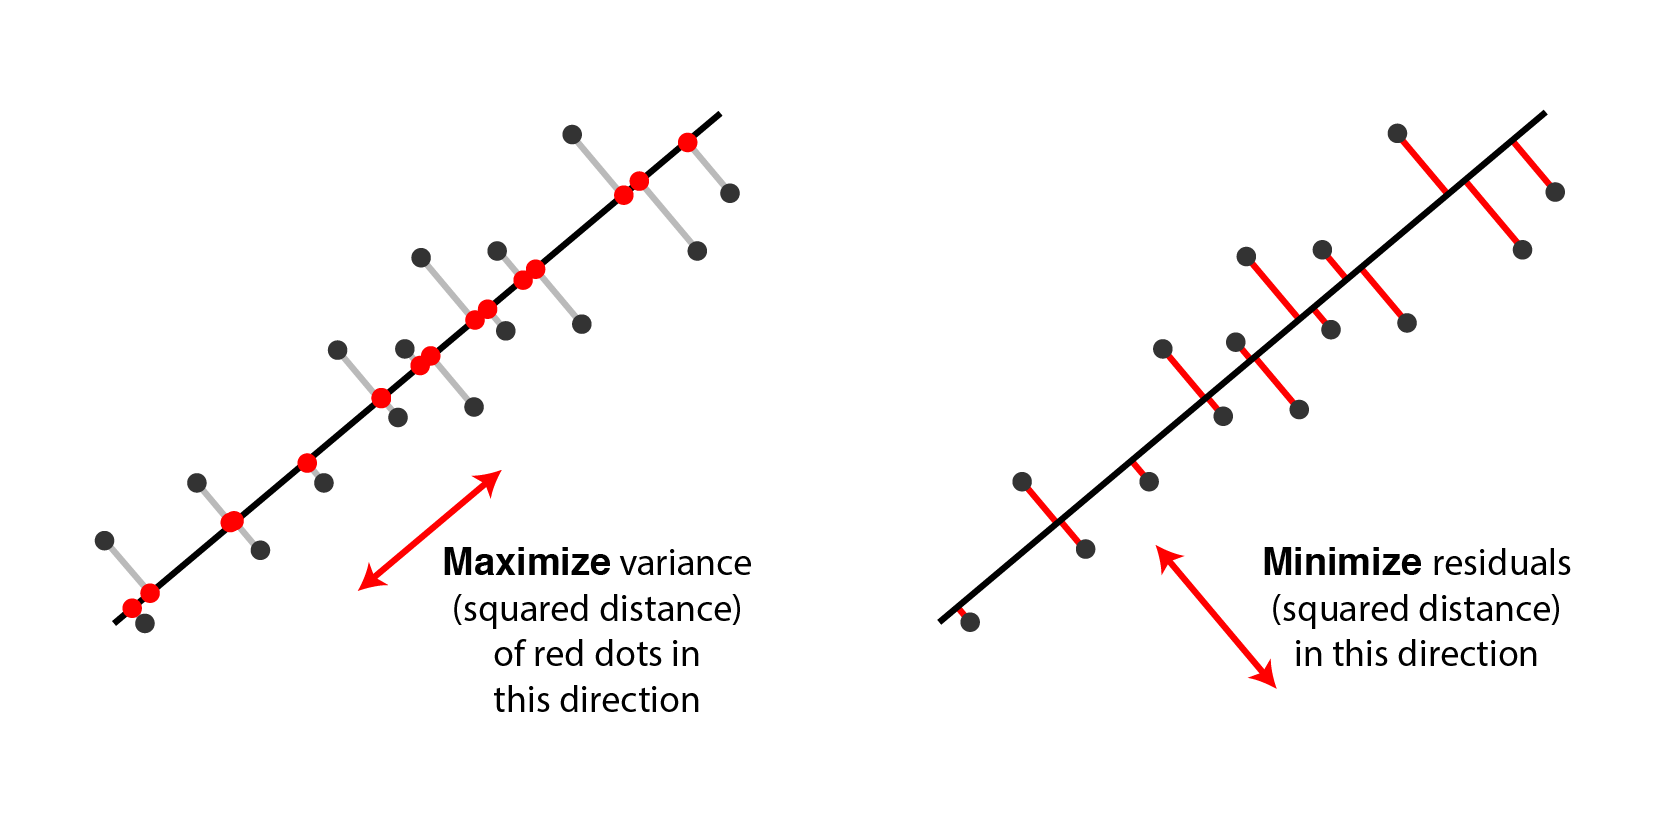
\includegraphics[width=1\linewidth]{resources/pcaDvaPogleda.png}
  \caption{Varianca in napaka rekonstrukcije. Vir:~\cite{quora_pca_explanation}}\label{fig:varerr}
\end{figure}
\begin{comment}
https://alexhwilliams.info/itsneuronalblog/img/pca/pca_two_views.png
\end{comment}
Dokažimo zgornjo trditev.
\begin{trditev}
  $u_{1} = \underset{u:\|\mathbf{u}\|_2=1}{\operatorname{argmin}}\ E(u) = \underset{u:\|\mathbf{u}\|_2=1}{\operatorname{argmax}}\ \operatorname{Var}(u^{\top}X^{\top})$
\end{trditev}
\begin{dokaz}
  \begin{equation}
    \mathbf{u_{1}} = \underset{\mathbf{u}:\|\mathbf{u}\|_2=1}{\mathrm{argmin}} \frac{1}{m} \sum_{i=1}^{m} \left\| \mathbf{u}^{(i)} - (\mathbf{u}^T \mathbf{x}^{(i)})\mathbf{u} \right\|^2
  \end{equation}
  \begin{equation}
    = \underset{\mathbf{u}:\|\mathbf{u}\|_2=1}{\mathrm{argmin}} \frac{1}{m} \sum_{i=1}^{m} \left\| \mathbf{x}^{(i)} \right\|^2 - (\mathbf{u}^T \mathbf{x}^{(i)}){}^2
  \end{equation}
  \begin{equation}
    = \underset{\mathbf{u}:\|\mathbf{u}\|_2=1}{\mathrm{argmax}} \frac{1}{m} \sum_{i=1}^{m} (\mathbf{u}^T \mathbf{x}^{(i)}){}^2
  \end{equation}
\end{dokaz}~\cite{gormley2018pca} \\
\begin{comment}
http://www.cs.cmu.edu/~mgormley/courses/606-607-f18/slides606/lecture11-pca.pdf
\end{comment}
Če enačbo za varianco malenkost preoblikujemo, dobimo naslednje.~\cite{zupan2024uozp}
\begin{equation}
  \begin{aligned}
    \mathrm{Var}(u_1^T X)
     & = \frac{1}{m} \sum_{i=1}^{m} \left( (u_1^T x^{(i)} - u_1^T \bar{x}){}^2 \right)                                                       \\
     & = \frac{1}{m} \sum_{i=1}^{m} \left( (u_1^T x^{(i)}){}^2 - 2 u_1^T x^{(i)} \cdot u_1^T \bar{x} + (u_1^T \bar{x}){}^2 \right)           \\
     & = \frac{1}{m} \sum_{i=1}^{m} u_1^T \left( x^{(i)} (x^{(i)}){}^T - 2 x^{(i)} \bar{x}^T + \bar{x} \bar{x}^T \right) u_1                 \\
     & = u_1^T \underbrace{\left( \frac{1}{m} \sum_{i=1}^{m} (x^{(i)} - \mu)(x^{(i)} - \mu){}^T \right)}_{\text{Kovariančna matrika } C} u_1
  \end{aligned}
\end{equation}
Zgornjo maksimizacijo variance lahko pod pogojem, da je $u_1$ enotski vektor, rešimo s pomočjo Langrangeovih multiplikatorjev.
\begin{equation}
  f(u_1) = u_1^T C u_1 + \lambda_1 (1 - u_1^T u_1)
\end{equation}
\begin{equation}
  \frac{\partial f(u_1)}{\partial u_1} = C u_1 - \lambda_1 u_1 = 0
\end{equation}

Po preoblikovanju enačbe, sledi da so to rešitve ravno lastni vektorji kovariančne matrike.
\begin{equation}
  C u_1 = \lambda_1 u_1
\end{equation}
Če zgornjo še malo preoblikujemo, ugotovimo, da lastni vektor z največjo lastno vrednostjo ohranja največ informacije o originalnem prostoru.
\begin{equation}
  u_1^T C u_1 = u_1^T \lambda_1 u_1 = \lambda_1 u_1^T u_1 = \lambda_1
\end{equation}
Podobno lahko za ostale nove bazne vektorje izberemo ostale lastne vektorje kovariančne matrike z najvišjimi lastnimi vrednosti.

Opazimo lahko tudi, da je kovariančna matrika simetrična $\Sigma = \Sigma^T$, zato bodo lastni vektorji ortogonalni, torej preslikava, ki smo jo dobili je samo rotacija originalnega prostora.

\section{Rešitev z uporabo SVD}
Lastne vektorje kovariančne matrike C lahko izračunamo s pomočjo singularnega razcepa.~\cite{zupan2024uozp}
\begin{equation}
  C = U \Sigma V^T
\end{equation}
Nato prvih k lastnih vektorjev vstavimo v matriko
\begin{equation}
  P = [u_1, u_2, \dots, u_k]
\end{equation}
Z matriko $P$, lahko sedaj preslikamo originalne podatke v nižje k-dimenzionalni prostor.
\begin{equation}
  y_i = P^T (x_i - \mu)
\end{equation}